\section{Hybrid-Driven Testing}

Hybrid-driven testing is the most commonly adopted automated testing technique
and consists in the combination of distinct features from two
or more automated testing techniques~\cite{Srinivas2017}. The most used combination is a mix
of the best features from both data-driven and keyword-driven testing
techniques. The combination of these automated testing techniques helps
the data-driven scripts take full advantage of the keyword-driven testing
libraries, leveraging the benefits of all the automated testing techniques.

\begin{figure}[!ht]
\centering
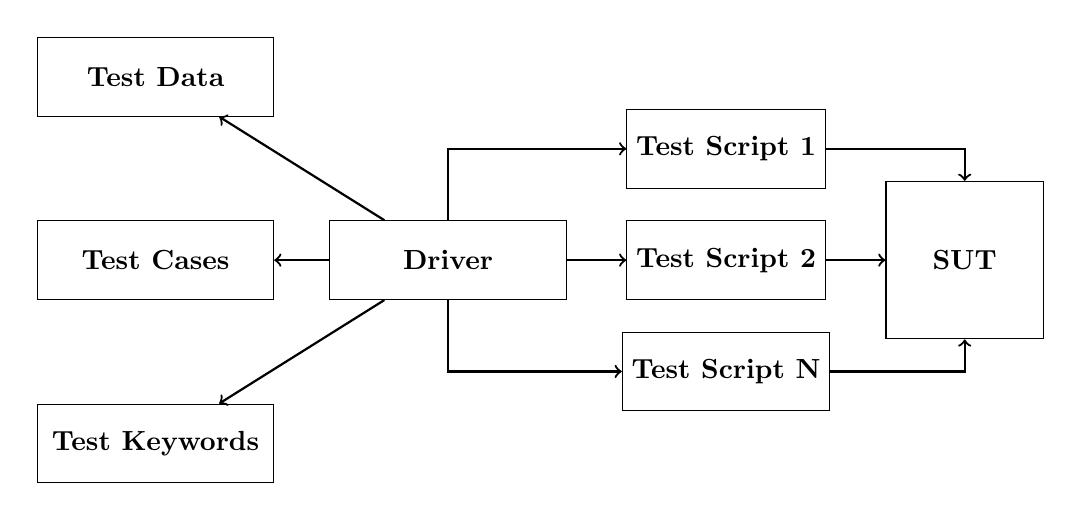
\begin{tikzpicture}
\matrix [column sep=7mm, row sep=-1mm] {
  \node (data1) [draw, shape=rectangle, minimum width=3cm, minimum height=1cm] {\textbf{Test Data}}; & & & \\
  &  & 
  \node (tscript1) [draw, shape=rectangle,minimum width=2cm,
  minimum height=1cm] {\textbf{Test Script 1}}; \\
  \node (parser) [draw, shape=rectangle,
  minimum width=3cm, minimum height=1cm] {\textbf{Test Cases}}; & \node (driver) [draw, shape=rectangle,
  minimum width=3cm, minimum height=1cm] {\textbf{Driver}}; &
  \node (tscript2) [draw, shape=rectangle,minimum width=2cm,
  minimum height=1cm, align=left] {\textbf{Test Script 2}}; &
  \node (sut) [draw, shape=rectangle, minimum width=2cm,
  minimum height=2cm] {\textbf{SUT}}; \\
  & & 
  \node (tscriptn) [draw, shape=rectangle,minimum width=2cm,
  minimum height=1cm] {\textbf{Test Script N}}; \\
  \node (datan) [draw, shape=rectangle, minimum width=3cm, minimum height=1cm] {\textbf{Test Keywords}}; & & \\
};
\draw[->, thick] (driver) -- (data1);
\draw[->, thick] (driver) -- (datan);
\draw[->, thick] (driver) -- (parser);
\draw[->, thick] (driver) |- (tscript1);
\draw[->, thick] (driver) -- (tscript2);
\draw[->, thick] (driver) |- (tscriptn);
\draw[->, thick] (tscript1) -| (sut);
\draw[->, thick] (tscript2) -- (sut);
\draw[->, thick] (tscriptn) -| (sut);
\end{tikzpicture}
\caption{Hybrid-driven system design approach that make usage of test data, test cases, and keywords in order to execute automated tests.} \label{fig:hybrid-driven-approach}
\end{figure}

With hybrid-driven testing, developers and testers can compensate the disadvantages
of using a single automated testing approach. It is designed to satisfy an organization
most wide-ranging automation requirement covering multiple applications, platform and environments.
This approach is suitable for big testing situations that have changeable data sets and
data transitioning cases. Normally, provides a good support for testing teams.

The goal is to make the testing scripts more compact and with a low chance of failure,
and facilitate the gradual conversion of testing scripts to keyword-driven equivalents,
when its necessary.

The hybrid-driven testing was designed around a set of important characteristics such as:
\begin{itemize}
\item \textbf{Maintainability}: tries to significantly reduce the test maintenance effort;
\item \textbf{Reusability}: due to the modularity of test cases and library functions;
\item \textbf{Conformity}: effective test design, execution, and traceability;
\item \textbf{Accessibility}: to design, develop & modify tests whilst executing;
\item \textbf{Availability}: scheduled execution that can run continuously;
\item \textbf{Reliability}: due to advanced error handling and scenario recovery;
\item \textbf{Flexibility}: framework independent of the system under test;
\item \textbf{Measurability}: customizable reporting of test results that ensure testing quality;
\end{itemize}

\subsection{Advantages of hybrid-driven testing}

The hybrid-driven testing is one of the most comprehensive testing techniques. It is a blend of the best features of other testing automation techniques.
It shares values of high usability, re-usability and test flow coverage offer built-in consistency and severity validation. Is easy to implement, easy to use, easy to expand, and easy to maintain. Shares the same high abstraction and like the keyword-driven approach is tool independent. When it is implemented it improves the speed of automating the test cases with the help of reusable libraries and provides better cost benefits.

\subsection{Disadvantages of hybrid-driven testing}

The biggest disadvantage of this approach is the need of an upfront investment in development and skills for the design, implementation and maintenance of the testing framework. By combining both data-driven and keyword-driven techniques, it is normal that the solution becomes even more complex but the flexibility that provides compensate the negative side of it.

\newpage